Our approach to the problem is the following:\\
We create a source node, and to this we connect $n$ nodes each representing one of the $n$ persons sharing the wash machine (lets call those nodes $P_i$ , $i$ ranging from 1 to $n$). The connecting edges between the source and the $P_i$ nodes initially have all a capacity of l. Then we create a sink node and to this node we connect $m$ nodes that represent the available time slots (lets call those nodes $T_j$ , $j$ ranging from 1 to $m$). All edges connecting the time slots with the sink have a capacity of 1. Then we connect each $P_i$ node with all the $T_j$ nodes that are included to this person's candidate list, again with edges of unitary capacity. When this process is complete, we have our network (Figure \ref{fig:prob3}).\\
\begin{figure}[ht]
\centering
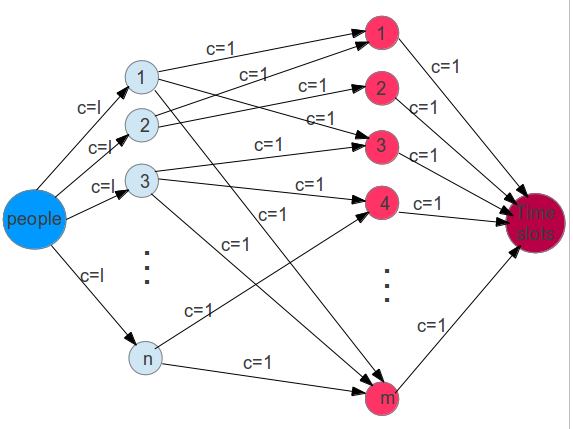
\includegraphics[width=0.75\textwidth]{prob3}%
\caption{Our network flow}%
\label{fig:prob3}%
\end{figure}
\\
We apply to the network that we created with the above mentioned procedure, the Ford-Fulkerson algorithm to find the maximum flow of the network. If we can get a maximum flow of $n*l$ that implies that there is a minimum valid assignment (meaning that every person gets the mimimum time slots among the ones in his list). If there is such an assignment and if $k$ is greater than $l*n$ we proceed as following:\\
We update each node's capacity to $h$, and then we apply an algorithm to find ${k-n*l}$ augmenting paths within our network, so that we get a network with flow equal to $k$. However, we apply the algorithm using one condition: that there can be no paths that go from a $P_i$ node to the source and then back to a $P_i$ node because there is a chance that then the corresponding edge's flow may be decreased below $l$, a fact that is undesirable according to the problem description.\\
If we find the desired number of augmenting paths then our goal is fulfilled otherwise, it cannot be reached. The cost of the algorithm is the sum of the cost of the maximum flow algorithm and the augmenting paths algorithm. Using the Ford-Fulkerson algo for the maximum flow, and the Edmonds-Karp for the augmenting paths, we get a complexity of O($V*$max(flow))+O($VE^2$) = O($V*n*l$)+O($V*E^2$) which is polynomial since the number of edges is bound by some multiple of $n$.
